\documentclass[conference]{IEEEtran}
\IEEEoverridecommandlockouts
% The preceding line is only needed to identify funding in the first footnote. If that is unneeded, please comment it out.
\usepackage{cite}
\usepackage{amsmath,amssymb,amsfonts}
\usepackage{algorithmic}
\usepackage{graphicx}
\usepackage{textcomp}
\usepackage{xcolor}
\def\BibTeX{{\rm B\kern-.05em{\sc i\kern-.025em b}\kern-.08em
    T\kern-.1667em\lower.7ex\hbox{E}\kern-.125emX}}
\begin{document}

\title{Procedural generation of levels for the angry birds videogame using
evolutionary computation\\
}

\author{\IEEEauthorblockN{ Jaime Salinas-Hernández}
\IEEEauthorblockA{\textit{Department of Graduate Studies} \\
\textit{Tijuana Institute of Technology}\\
Tijuana, México \\
salinas.jaime1217@gmail.com}
\and
\IEEEauthorblockN{ Mario Garcia-Valdez} \IEEEauthorblockA{\textit{Department of Graduate Studies} \\
\textit{Tijuana Institute of Technology}\\
Tijuana, México \\
mario@tectijuana.edu.mx}
\and
\IEEEauthorblockN{ JJ Merelo} \IEEEauthorblockA{\textit{Department of Graduate Studies} \\
\textit{Universidad de Granada}\\
Granada, Spain\\
jmerelo@ugr.es}}

\maketitle


\begin{abstract}
    % We do not say this project, is more like: In this paoer an evolutionary ... 
    % is presented or In this paper we present a .... (in third or first person plural) - MG   
    In this paper an evolutionary computation-based system is proposed to generate 
    levels for the Angry Birds video game, the levels themselves are composed of a 
    set of birds that the player can use, a certain amount of pigs that must be destroyed 
    in order to progress to the next level and a given number of pieces that conform 
    structures that may or may not protect the pigs from the player. The focus in this stage
    is the generation of diverse structures that can be played in the game having the
    additional characteristics of being interesting and playable. We propose a 
    multi-layered search, first contructing composite structures from basic components, to then
    build more complex structures building from these components, following an open-ended 
    evolution approach; in which the evolution of structures is not guided towards 
    a single objective but rather is free to evolve and generate novelty or diversity. 
    The objective is then that the proposed levels are evaluated by how complex they become and how 
    different they are from the rest of the group. The experiments conducted show that a evolutionary approach allows the generated levels
    to have a level of uniqueness because on most of the cases the way they are presented on screen
    is a way a normal human would have trouble to create but at the same time are interesting to see.
    % Maybe like this ? JSH
    %The experiments conducted show  
    % We found that in the experiments conducted, levels generated where ...  
    
    % The abstract is not only for stating what whas done, it is also for 
    % telling readers, why they should care, what's novel, how good it is, how you tested.
    % Please get some inspirtation from other abstracts on the same subject,
    % this should be the last section we write. - M  
    \end{abstract}
    
    \begin{IEEEkeywords}
    genetic algorithm, procedural generated content, open-ended evolution,
    evolutionary computation
    \end{IEEEkeywords}
    
    \section{Introduction}
    Procedural content generation is an interesting subject on the entertainment
    industry, primarily in video game development because of the savings in 
    time and human resources when generating content for different video game projects \cite{Yannakakis2017,YannakakisContentGeneration}.
    In this paper an evolutionary content generation system is proposed to generate
    levels for the popular Angry Birds video game,
    taking inspiration in concepts of open-ended evolution. Angry birds is a game 
    developed by Rovio Entertainment in which the objective is to destroy structures
    placed on the map as well as eliminating
    green pig-like entities in order to obtain the highest score possible, the game
    uses a gravity and collition system that allows the structures to fall and be
    destroyed by means of damage as well as the use of three different construction
    materials \textit{ice}, \textit{wood} and \textit{stone} each one with a different
    resistance, ranging from fragile, normal and sturdy in that order. The game
    mechanic is to use a slingshot to shoot a certain number of birds with different
    abilities, to destroy both the structures and the objectives. A high score 
    is achived by doing the most destruction with the least birds possible 
    \cite{RovioEntertainmentCorporation2009}.
    
    %While it is possible to create an evolutionary agent to play the levels and
    %obtain the best score 
    The main objective of this project is to generate levels that can be played
    by naïve or inteligent agents as well as physical players. The levels
    themselves need to be complex in the sense that interesting structures can be
    created, but at the same time, it is possible to complete in some way
    \cite{Stephenson,Stephenson2018}.
    
    % What is the problem?
    Procedural content generation provides a peculiar case of study because of the
    way
    % Is there a reference? - MG
    content has to be made for a each particular type of game. In this use case we
    have those restrictions dictated by the game, and also those imposed by a
    competition track \cite{Renz}.% Reference the paper of the competition  have
    provide an interesting The challenge for the participating algorithms is to be
    flexible on the pieces that can be used and the runing time of the algorithm, as
    they are determined at runtime. 
    %their interactions with one another because of gravity and the possible effects
    %the trajectory of a shot from a player can affect all of this. How we solve it?
    %(summary)   
    In order to tackle this case study, we proposed the use a genetic algorithm capable 
    of creating game levels having the objective of being both \textit{interesting} and 
    \textit{playable}, the way to test our candidate solutions will be by using a open-source
    software called Science Birds \cite{sciencebirds} which uses the same resources used on the
    original angry birds game.
    
    % What is learned?
    In this work we found that an evolutionary algorithm can be used to create 
    this type of content not only because it is able to create levels that are interesting 
    and diverse but because an evolutionary algorithm is capable of creating things a 
    normal human could have trouble imagining of.
    
    % What is learned?
    %We identify the places were an evolutionary algorithm can be used alongside
    %procedural content generation applied to video games in order to be able to
    %clarify in which areas an evolutionary algorithm can used to further improve
    %video game development cycles.
    
    % En este trabajo se generan estructuras con mayor diversidad y por lo tanto 
    % resultan ser interesantes.
    
    We propose a basic Open-Ended Evolution (OEE) algorithm, a variant of genetic
    evolution algorithm where the objective differs from that of a regular genetic
    algorithm,  in this case the final objective is not to reach a final state of
    the evolution (an optimal solution) but to continue evolving and creating new
    types of entities, perhaps more complex on each new generation. Solutuion
    entities have the possibility to evolve not only inside the frame of their type,
    but  they can create entirely new groups \cite{Standish2003}. Taylor et al.
    \cite{Taylor2016,Taylor} defines OEE as a system capable of creating novelty
    beyond a point where nothing changes on the current group of interest rather
    than just converging to a stable or quasi-stable state.For this project, OEE is
    defined simply as a genetic evolution process with different clasess of objects,
    with compositional and taxonomic relationships between them. Objects of each
    class can evolve in parallel or as in this case, independenly of each other. The
    idea is based on the object oriented model, in which complex behavior can be
    model using these principles. The rest of the paper is as follows.
    
    %% TO DO: This needs to be adjusted to the final version. We need to use
    % \ref for the numbers - MG
    
    Section 2, contains a quick overview of some aspects used by different authors
    in order to tackle this problem, their design and basic functionality, in
    Section 3 the description of the current state of the project is explained, from
    %% The following sentence is not clear.
    the way the candidate solutions are represented, to the way the mutations are applied 
    to them, as well as the way we use our fitness fucntion to determine the playability
    and complexity of the generated levels, 
    %the basis of the development, modification to the original proposed method as 
    %well as different approaches that were taken to solve the problem.
    % to the different methods that have been used to
    %progress on the different sections of the project, 
    % Normaly there is no "Future Work" section is put together with Conclusions - MG
    finally in Section 4 we provide our conclusions about the development of this
    paper as well as improvements that can help to refine the proposed work. 

    %Maybe like this? JSH
    
    %we explain the future work of the project, where we are in the development phase and how the
    %future implementations are to further improve the project and finally, in
    %Section 6 we present our conclusions
     
    
    
    %\section{Background}
    %
    %In this Section we provide a quick overview of the literature about the areas
    %that provide the basis to the development of the current project, this section
    %is divided in three parts, the fisrt one gives us an explanation of what
    %procedural content generation entails, the second one provides an explanation on
    %genetic algorithms and how can they be used to solve optimization problems, and
    %finally, the third one provides us with an overview of open-ended evolution and
    % use just one form, I prefer with no first caps open-ended evolution and let's 
    % use an abbreviation OEE - MG 
    
    %what it means to have an open-ended evolution algorithm.
    % For this conference I think we do not need to define PCG, let's think 
    % every one knows what it is. - MG 
    
    %\subsection{Procedural content generation}
    
    %Procedural content generation (PCG) 
    
    %\subsection{Genetic algorithm}
    
    
    
    
    % This section and the proposed approach should be in the fron lines - MG
    
    % The problem is that we just state what it is, but we do not link it
    % with our work. Why is important? What inpired our work? 
    % There is also Novelty Search - MG
    % Also it sounds like a copy-paste from Wikipedia please check and reference
    % accordingly - MG
    
    %\subsection{Open-Ended Evolution}\label{AA}
    
    
    \section{State of the art}
    \label{SoA}
    In this Section we present PCG works relevant to the Level generation for the
    Angry Birds video game. Renz et al. \cite{Renz, Renz2015TheAB} organized an AI
    competition with the aim of developing intelligent agents that could play new
    Angry Birds levels better than the best human players. The competition was then
    collocated in other AI conferences. In order to train and test these agents,
    more novel and some times difficult levels must be generated. A related
    competition was then proposed by Stephenson et al. \cite{Stephenson} this time
    with the goal of developing a level generator for the game. Several generators
    have been proposed in the following years of competition. M. Kaidan et al.
    \cite{Kaidan2015} propose a model in which the generation of content is
    controlled by the skill of a player while actively playing the game, the moment
    the player finishes a certain level the algorithm obtains the score and
    generates the next level to be played. Y. Jiang et al. \cite{Jiang2017} proposed
    the use of predefined letter style patterns and combined to create a small pool
    of words and letters used to be combined in order to create levels with text on
    them, the participants would play the game and after that they would be asked if
    they liked the layout of the levels. A search based approach has been also used
    in several works. Laura Calle \cite{lauracalle} proposed a method in which the 
    pieces in the game are arranged in groups using the gravity of the game to 
    create structures that are later evolved into more complex levels, this method 
    was used as a base to work with since it used a modified version of the angry 
    birds game that was able to obtain the data of a level after a simulation.
    %%%
    % TO DO: Laura´s work here 
    %%%
    
    \section{Proposed Method}
    
    In this Section we describe the approach used in this work, explaining first,
    the restrictions of the game.
    The game contains a total of 11 block shapes as shown in Figure \ref{piece_list}.
    These basic blocks cannot be modified, it is not possible to add more or modify the existing ones,
    with this in mind the purpose is to create composites of these blocks in
    different locations and angles in order to create structures that can be used as
    building blocks for more complex structures. 
    
    \subsection{Composite Generation}

    Since there is no way to \textit{add} a new composite to the pool of blocks,
    then a way to combine both is needed, in order to do this first the original
    11 pieces of the game will be converted into composites of a single element.
    A composite is defined as a lists of blocks, then a \textit{composite} of
    one element will be created for each piece. Composites are the first layer
    the building blocks for the structures to come. A composite could include
    different types of blocks, rotaded at a certain angle and compose a basic
    structure. An ideal composite could support other composites on top with out
    falling apart, but this is not required. A composite is measured using
    maginary bounding box, defined by calculating the lengths of all the pieces,
    finding the borders of said pieces and then finding the points that could
    define a box around all of them, then use this defined box to calculate the
    height and width of the new composite and then calculate from the center
    point of said box the offsets from the center of the group to the center of
    each respective piece as shown on figure \ref{bounding_boc_calc}, this
    information is needed in order to add it as a new composite so it can be
    used to place the pieces in their respective new positions when the files
    needed for the simulation are being created. This is similar to creating a
    group of elements in a drawing application.

    %% 
    Good composites can be found using an evolutionary approach proposed earlier 
    by Calle and Merelo, where basic structures are generated by searching a space
    of falling blocks and selecting those that remain standing. This algorithm is 
    not capable of creating complex strucures, but it can generate very novel basic
    structures. We can see that the evolution at this level can benefit from having
    more freedom in how basic structures are built. We do not want to form piles
    or sequences of blocks, this will be done at a higher level in the composite hirarchy.
    
    At this level the composite generator has the following steps:
    
    % Pleas explain in more detail this Composites in a section.  
    % Here it's explained better, maybe this paragraph should be moved to
    % an earlier point - MG
    
    % Needs a few touches - MG
    % Please use the name Composite instead of Bundle, composition is well known in
    % object oriented design.
    
    %                                                                           /|\
    % Combined a few other things to give a litte more detail to this sections   |
    %                                                                           \|/
    
    \begin{enumerate}
    \item Generate the first generation of the population, consisting of
    randomly generated list of blocks.
    \item Run a Simulation.
    \item Evaluate each individual of the population.
    \item If a member of the population has remaining pieces obtain the location
    and angle of the pieces, assign a fitness.
    \item Do the selection, crossover and mutation operations.
    \item Repeat the cycle.
    \item From the best individuals select composites. Several algorithms could
    be proposed for this step, for instance selcting clusters of blocks.
    \end{enumerate}
    
    Another option is to just manually generate interesting composites to be used by the algorithm.
    We could say that the previous approach is an option for a procedural generation of composites.

    \begin{figure}[htbp]
    \centerline{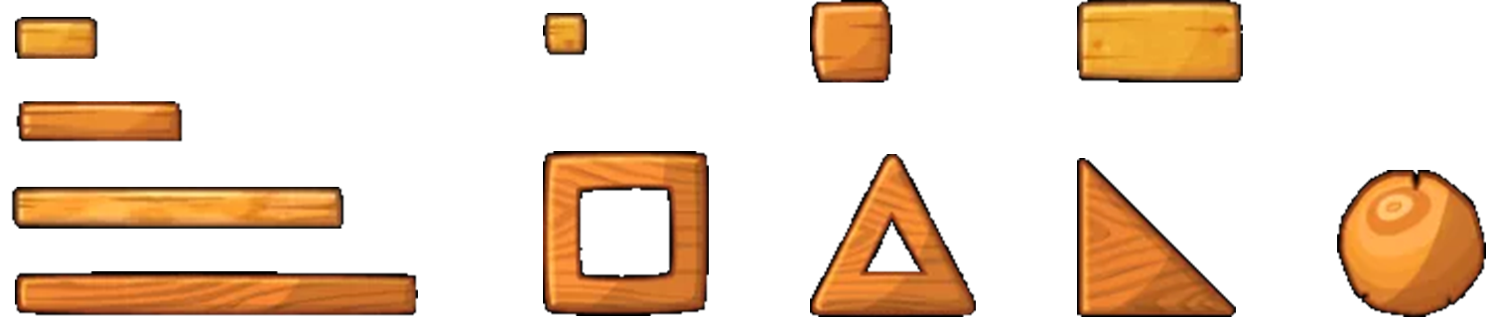
\includegraphics[width=80mm]{Images/list_pieces.png}}
    \caption{List of pieces in the angry birds game.}
    \label{piece_list}
    \end{figure}
    
    % Explain a bit about the competition, from the introduction
    
    The Angry Birds level generation track is a competition where the objective is 
    to generate levels that are \textit{fun} and \textit{enjoyable} however they 
    also have to be challenging but not imposible. However the rules for the competition 
    specify that a configuration file must be used to
    generate the levels of the game in a limited amount of time, the information on
    the configuration file is first the number of \textit{different} levels
    that must be generated, the second value is the different materials \textit{not
    allowed} to be used, for instance a group of generated levels must not have
    circles which composition material is ice or stone, moreover it does not have to
    integrate a triangle piece with ice, stone or wood material so this combinations
    must be removed from the pool of options, the third configuration value is the
    \textit{number of pigs} that must be placed in a level, and finally the
    \textit{limit} of time that the system has to create the required amount of
    levels.
    
    %After taking into account this restrictions the structure of our current approach
    %had to be changed, so this section will be divided in two subsections, the first
    %will explain the approach that was used and after that the second will explain the
    %modifications that had to be made in order to integrate the configuration files
    %for the competition. 
    
    In our original approach, composites could added to the structure generator
    algorithm at runtime as a mutation of an individual. The structure generator
    is explained in the next section.

    % Lets check this, I think is not needed. 
    %The objective in this first phase of the project was to
    %generate structures that were capable of maintaining their own balance as
    %shown on figure \ref{test_old}, since the objective of open-ended evolution
    %for this project is to add new composites to the pool of options,
    
    In our current approach the composite generator is only
    run once at the beginning, as a setup process.
    

    \subsection{Structure Evolution}
    % This sentence needs more work -MG

    %During the original phase of the design of the system, it was decided that the way 
    %composites were going to evolve was by first placing only base pieces on a level 
    %then after a simulation the remaining pieces
    %of a member of the population were going to be used as a new composite if after a 
    %simulation a group was still standing and grouped on a single point, their individual 
    %offsets from the center of the group was calculated and then using this information a new 
    %composite could be added to the pool of options, this new
    % we don't use member of the populations, use proposed solution, candidate solution
    % or individual of the population. - MG  
    %additions to the composite pool could then be added to the population by the mutation
    %operation when a new member of the population was being created, the objective 
    %in this first phase of the project was to generate
    %structures that were capable of maintaining their own balance as shown on figure
    %\ref{test_old}, since the objective of open-ended evolution for this project is
    %to add new composites to the pool of options, then the algorithm will first run a
    %simulation with a group of pieces and after it the ones that were not destroyed
    %by falling because of gravity will be saved and added to the pool of options.
    
    % New pieces are added by mutation? 
    % Please give more details to all this - MG
    

    
    \begin{figure}[htbp]
    \centerline{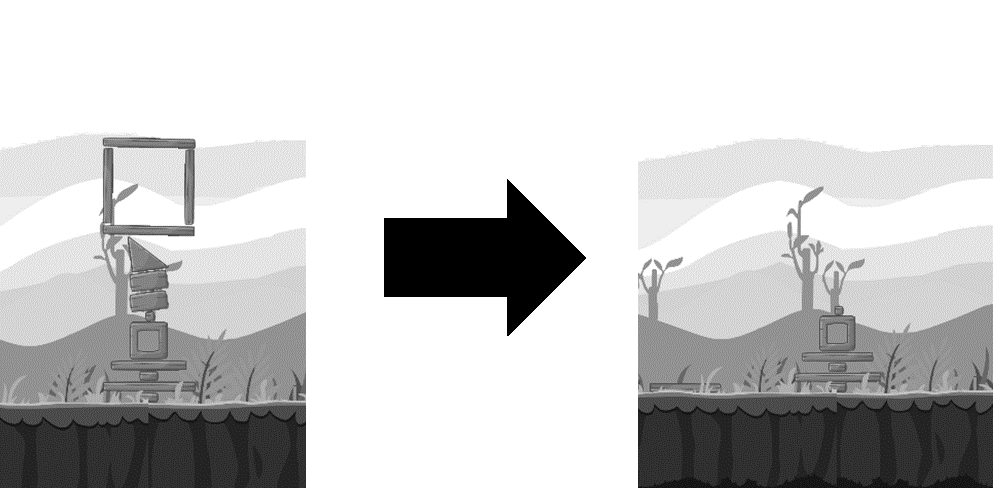
\includegraphics[width=80mm]{Images/simulation_bef_aft_example.png}}
    \caption{Structure at beginning and end of a simulation.}
    \label{test_old}
    \end{figure}
    
    Structures are the next evolutionary layer, at a higher level of composition.
    Structures are compositions of composites. A level can be seen as a collection 
    of structures and each structure is a pile of composite blocks. This approach 
    was proposed by \cite{ }. This way of constructing levels has the advantage of
    limiting the search space, to structures that have a better chance to be 
    standing after the simulation ends. There is no warranty that piles of 
    composite blocks will maintain balance, so again we must search for those 
    structures.

    Structures are represented in a way similar to Togelius et al.
    \cite{togelius2016Representationsforsearch-basedmethods}. Each block has
    an id assigned to it. A structure is then a list of ids, refering to
    composite blocks, the first 11 are basic composite and generated composites 
    are assigned a higher number.  This way and individual can be
    represented as shown on figure \ref{old_chrom} where each chromosome
    represents a certain item in the list of blocks, the numbers for this
    elements are assigned in a first come first served basis, the numbers are
    infinitely incremented and the same blocks can be repeated in a structure.
    
    \begin{figure}[htbp]
    \centerline{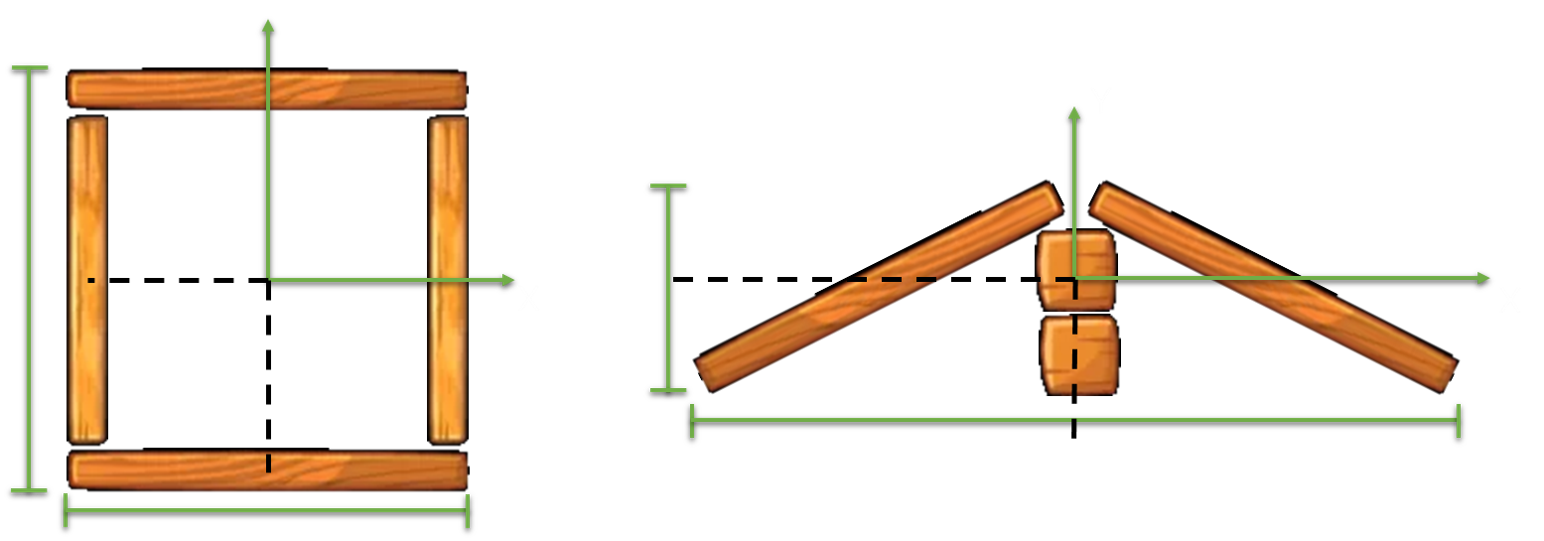
\includegraphics[width=80mm]{Images/bounding_box_calculation.png}}
    \caption{Bounding box calculation.}
    \label{bounding_boc_calc}
    \end{figure}
    
    \begin{figure}[htbp]
    \centerline{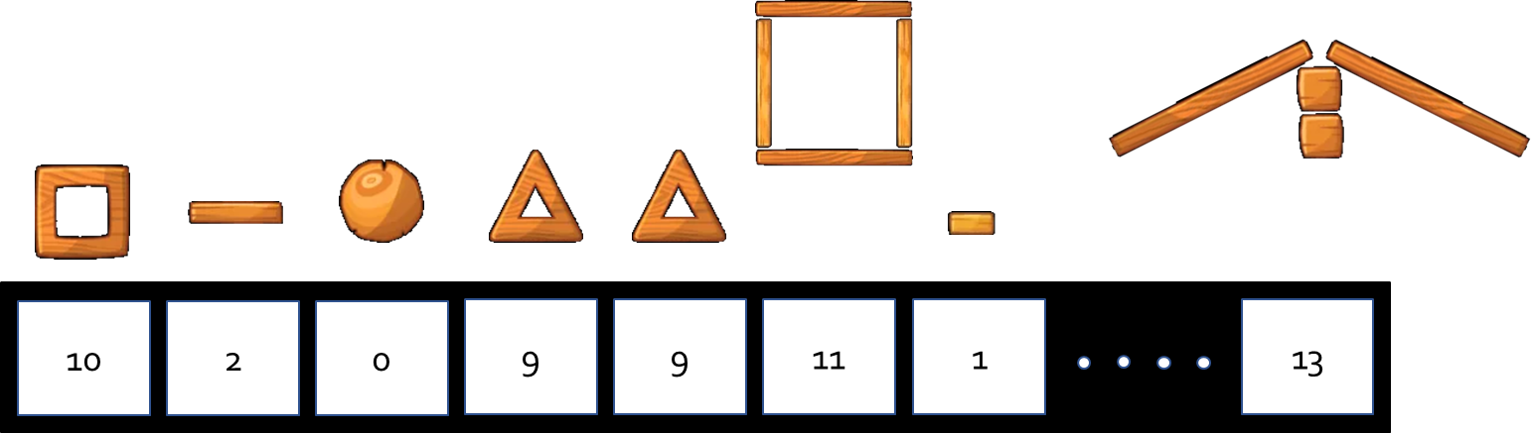
\includegraphics[width=80mm]{Images/chromosome_chain_example.png}}
    \caption{Chromosome chain of an individual.}
    \label{old_chrom}
    \end{figure}
    
    These structures represent individuals in the evolutionary algorithm. Once
    an individual is created it is ready to be evaluated in a simulation on the
    game environment. Using a similar approach as the composite generator, all
    individuals have a maximum of ten seconds to maintain balance or reach
    absolute stability, if absolute stability is reached it means one of two
    things, first the generated structure is completely stable or second, the
    tower fell to either side and the pieces were destroyed or stopped moving by
    gravitational pull, when either of this happens by more than two seconds the
    simulation ends regardless of time remaining and the next individual is
    simulated.

    The evaluation process for this project is still in the development stages,
    and in our experience is one one of the more difficult components in this
    kind of systems. In this stage of the evolution, we first need to assign a
    good fitness to those structures that keep their balance and not fall apart.
    There are other variables we take in to account, but they will be explained
    later. In this initial stage, each individual in the population has 100
    points so before the simulation starts each of them are viable candidates to
    be an elite member of the population regardless of their relative height or
    complexity.
    
    First, after each of the individual simulations are over the evaluation process
    takes place, in this phase the resulting level is checked for those blocks that
    survived, that is they where not destroyed by falling. Each one
    of them is counted and then the resulting number is compared to that of the
    initial quantity of pieces that were originally put in before the simulation,
    each block represents a certain percentage of 100\% so the missing pieces 
    are subtracted from the total. In this moment, each block is counted as if 
    it was not a member of a composite, this is becuse after the simulation there is
    only data about each individual block.  
    
    %Second, after removing a percentage according to the missing pieces an individual
    %remaining pieces are checked for their positions in comparison to the original
    %ones before the simulation, using the formula 1 each piece within the individual
    %is evaluated according to the center point of the piece, if the piece moved more
    %than a certain threshold half the percentage for one piece is removed from the
    %remaining percentage, after this using formula 2 the position of the piece
    %is further checked, this time by the difference in angle from the original one,
    %in case the difference of angles is more than a certain threshold half a piece
    %value is further removed from the total.
    
    %\begin{equation}
    %    \begin{aligned}
    %    error_{xy} = \left\{ \,
    %        \begin{IEEEeqnarraybox}[][c]{l?s}
    %            \IEEEstrut
    %            0.1 & if $ 0.08 > d $, \\
    %            \frac{100}{lenght\_pieces} * 0.5 & if $ 0.08 < d $.
    %            \IEEEstrut
    %        \end{IEEEeqnarraybox}
    %    \right. \\
    %    where: d=\sqrt{(x_2 - x_1)^2 + (y_2 - y_1)^2}    
    %    \end{aligned}
    %    \label{error_xy}
    %\end{equation}
    
   % \begin{equation}
   %     \begin{aligned}
   %     error_{r} = \left\{ \,
   %         \begin{IEEEeqnarraybox}[][c]{l?s}
   %             \IEEEstrut
   %             0 & if $ -5 \le r \le 5 $, \\
   %             \frac{100}{lenght\_pieces} * 0.5 & if $ r < 5 \: or \: r > 5 $.
   %             \IEEEstrut
   %         \end{IEEEeqnarraybox}
   %     \right. \\
   %     where: r= |rotation_0| - |rotation_f|   
   %     \end{aligned}
   %     \label{error_angle}
   % \end{equation}
    
  % Finally, the total height of the remaining group of pieces is calculated by
  %  combining the bonding boxes of all pieces, then the individuals are ordered by
  %  the obtained percentage and then further ordered by the total height, this way
  %  the most balanced ones will have the best probability to be selected together
  %  for a crossover operation to create the next generation.
    
 %   \begin{figure}[htbp]
 %   \centerline{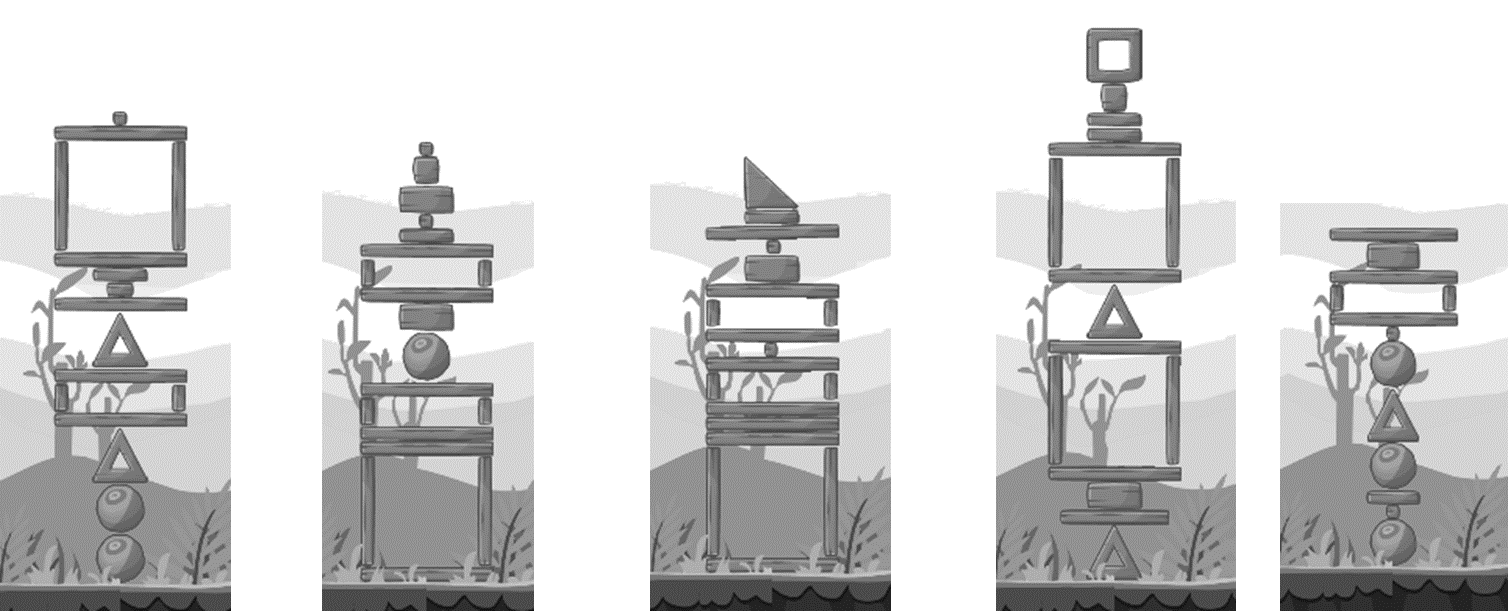
\includegraphics[width=80mm]{Images/result_example.png}}
 %   \caption{Result samples of current system.}
 %   \label{results_old}
 %   \end{figure}
    
 %   Since there is a need to create complex structures than can cover a great
 %   section of the play map, a method to evaluate the distribution is needed, for
 %   this instance we propose using the rule of thirds \cite{DarrenRowse} which is a
 %   guideline used while creating images, the purpose is to create
 %   aesthetical pleasant images where the focus point or the most important area is
 %   at the center of the image as shown on figure \ref{rule_of_thirds}, using this
 %   rule different distribution groups or masks are created has shown on figure
 %   \ref{rule_of_thirds_masks} in order to use them before the simulation of an
 %   individual by placing the pieces in order to distribute them in a way that can cover
 %   more area and create more balanced levels instead of using a tower like
 %   distribution as shown on figure \ref{results_old}.
    
 %   \begin{figure}[htbp]
 %       \centerline{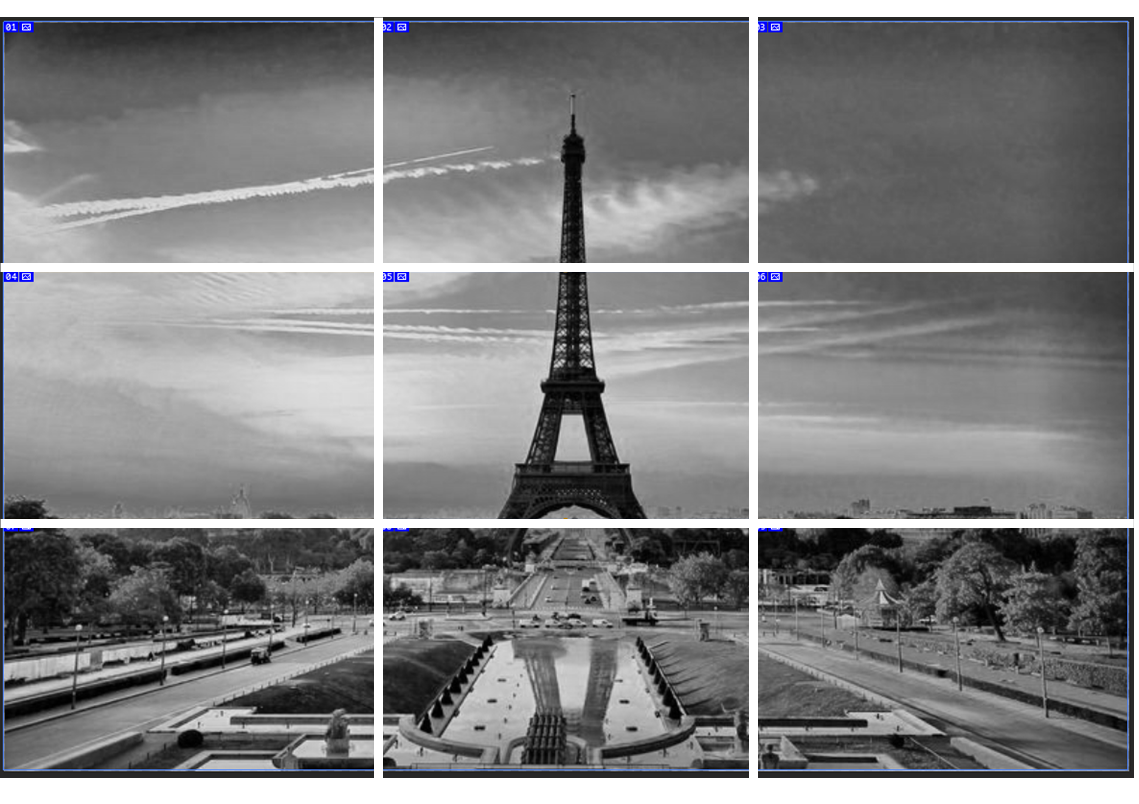
\includegraphics[width=80mm]{Images/ruleofthirds_example.png}}
 %       \caption{Rule of thirds example.}
 %       \label{rule_of_thirds}
 %   \end{figure}
    
 %   \begin{figure}[htbp]
 %       \centerline{
\includegraphics[width=80mm]{Images/mask_distribution.png}}
 %       \caption{Masks created using the rule of thirds.}
 %       \label{rule_of_thirds_masks}
 %   \end{figure}
    
    Using this same distribution a new evaluation will be added in which according
    to how much of the area is filled a score will be given and this score will be
    used as a new sorting value at the moment of selecting individuals for the
    crossover operation, since as shown on figure \ref{rule_of_thirds_masks} there
    is a possibility that a huge mask is given to an individual it can be possible
    that the amount of pieces will not be able to cover the full area given, so in
    order to prevent this kind of problem we also proposed to give each mask a
    value that refers to the minimum amount of pieces and height required to fill
    the most of the mask, then check the amount of pieces and height before
    simulation for a single individual and then randomize which mask of the ones
    that can be used will be assigned to that individual, this way the results shown
    on figure \ref{rule_of_thirds_result} are obtained, this however gave us a new
    problem because as shown in the figure and on figure \ref{rule_of_thirds_applied} as well, the were
    instances in which a certain combination of pieces could be to big for the area
    and this pieces resulted in a level that had structural flaws from the beginning
    which cold provoke the entire structure and immeadiately nearby others to fall
    at the beginning of the simulation however this allowed us to realize that predefined 
    composites could provide problems to the generated structures therefore this approach 
    was not the best for this problem.
    
    \begin{figure}[htbp]
        \centerline{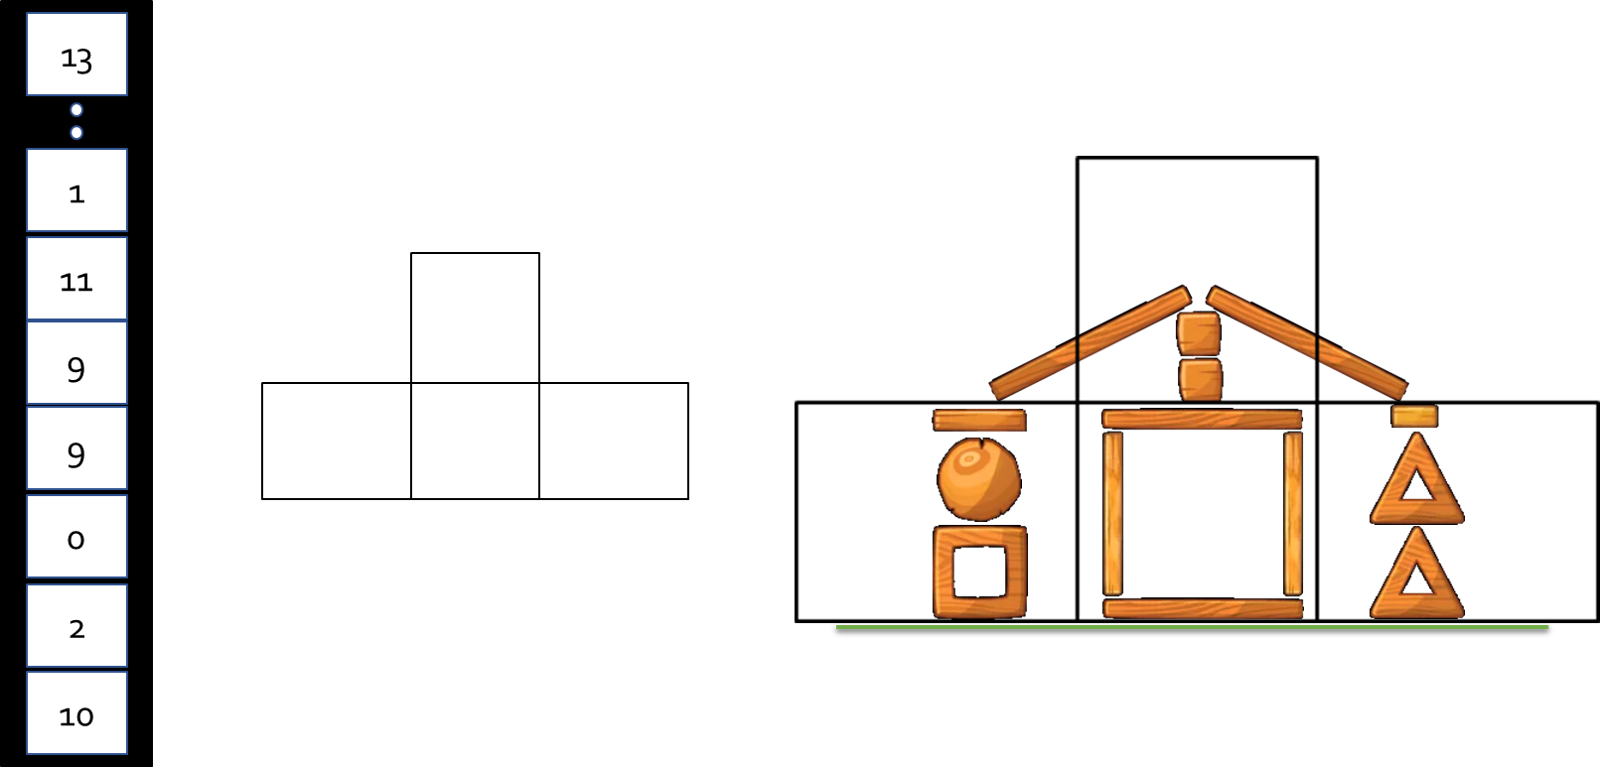
\includegraphics[width=80mm]{Images/chromosome_thirds.png}}
        \caption{Rule of thirds applied to an individual.}
        \label{rule_of_thirds_applied}
    \end{figure}
    
    \begin{figure}[htbp]
        \centerline{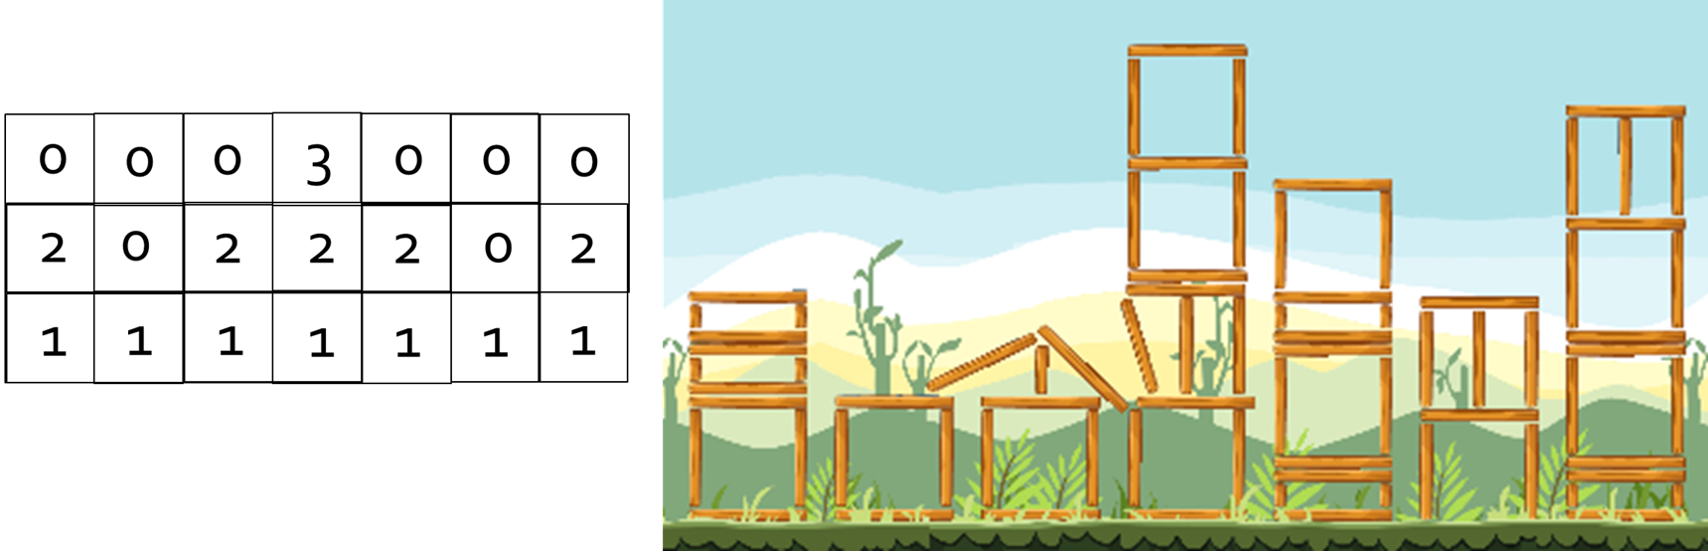
\includegraphics[width=80mm]{Images/result_example_thirds.png}}
        \caption{Results obtained with rule of thirds.}
        \label{rule_of_thirds_result}
    \end{figure}
    
    \subsection{New approach}
    
    The first differece that the new approach has is that the masks that are assigned
    to each individual are no longer pre-generated ones, this is because we decided
    that pre-generating them would not allow the generator to \textit{evolve}
    because the individuals would be limited to a certain number of possibles
    combinations which will in turn prevent diversity in the population, so in order
    to prevent this the modification to this section allows the individuals to
    generate a mask in which a number of columns is defines by default but the
    amount of pieces in each one is random, however the total of assigned pieces in
    all columns must be the same as the total pieces allowed in each individual
    which is a number assigned before beginning the system, an example of this
    can be seen in figure \ref{new_chrom} where the total of pieces in a individual
    is 18 and this pieces are distributed on all the columns available. This is
    further explained in this section.
    
    The competition also requires that a generator follows a certain ruleset this is 
    emulated by providing a file to the system to simulate the ruleset provided at the 
    competition, this \textit{text file
    (parameters.txt)} provides the specifications that must be met in the
    competition, the parameters in the file are as follows:
    
    \begin{itemize}
        \item Total required levels.
        \item Restrictions to pieces or piece-material combinations that cannot be
        placed or used in the levels, in this case if the file specifies that a
        \textit{CIRCLE} made out of \textit{ICE} cannot be placed, so the system must be
        able to verify that said combination is not used.
        \item Total number of pigs, this value can be a single value or a range of
        values that represent how many pigs must be placed on a level.
        \item The amount of time in which the system must give an output.
    \end{itemize}
    
    \begin{figure}[htbp]
    \centerline{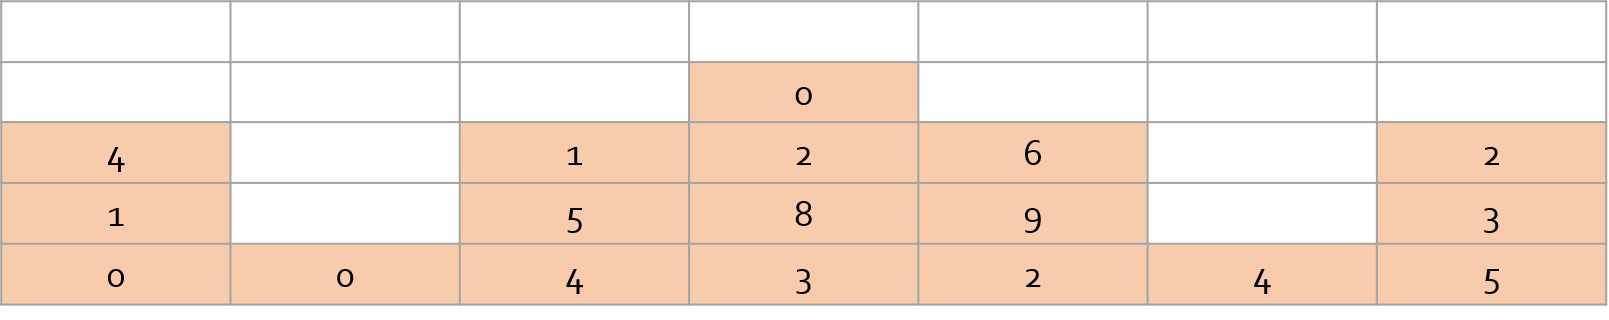
\includegraphics[width=80mm]{Images/chromosome_chain_new_model.png}}
    \caption{New chromosome chain.}
    \label{new_chrom}
    \end{figure}
    
    \begin{figure}[htbp]
    \centerline{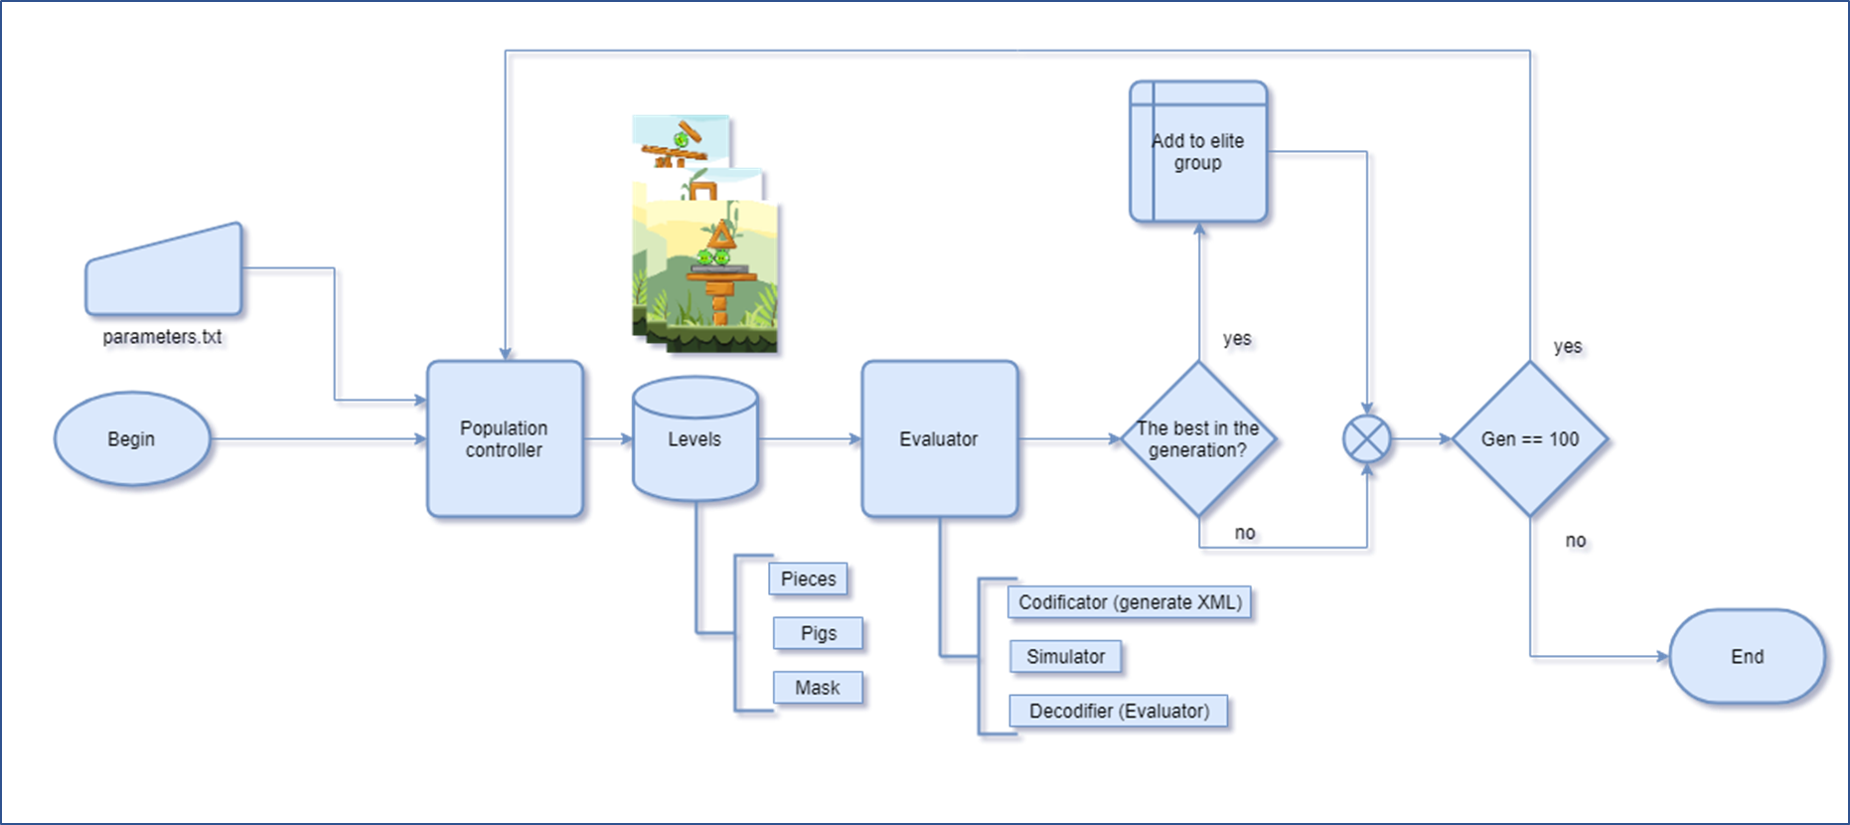
\includegraphics[width=80mm]{Images/new_model_v2.png}}
    \caption{New system diagram based on the parameter file and the new chromosome representation.}
    \label{new_model}
    \end{figure}
    
    Using this as a base a new system diagram is proposed as shown of figure
    \ref{new_model} in which the file with parameters is integrated with the input
    data  the system requires, the way the individuals of the population are further
    presresented and the way the simulation phase is taken, the method to
    representate the individuals is proposed by dividing the individual on three
    layers represented as follows:
    
    \begin{itemize}
        \item Element layer: also known as pieces layer, this layer represents the
        elements assigned to a particular individual by an array of numbers from 0
        to infinite, where each number represents a reference to the class of a piece
        in the selection pool including the ones generated by the OOE algorithm, the
        representetion of this is was shown in figure \ref{old_chrom}.
        \item  Mask layer: this layer is represented by a 7 digit array in which the
        value assigned in each column represents the amount of pieces from the
        element layer that will be assigned to said column, a representation of this
        is shown on figure \ref{mask_layer}.
        \item Enemy layer: also known as pig layer, this layer is represented by two
        elements a single numeric value representing the total amount of pigs
        assigned to the level and an array of locations for the placement of this
        same pigs, a representation of it is shown on figure \ref{enemy_layer}. 
    \end{itemize}
    
    \begin{figure}[htbp]
        \centerline{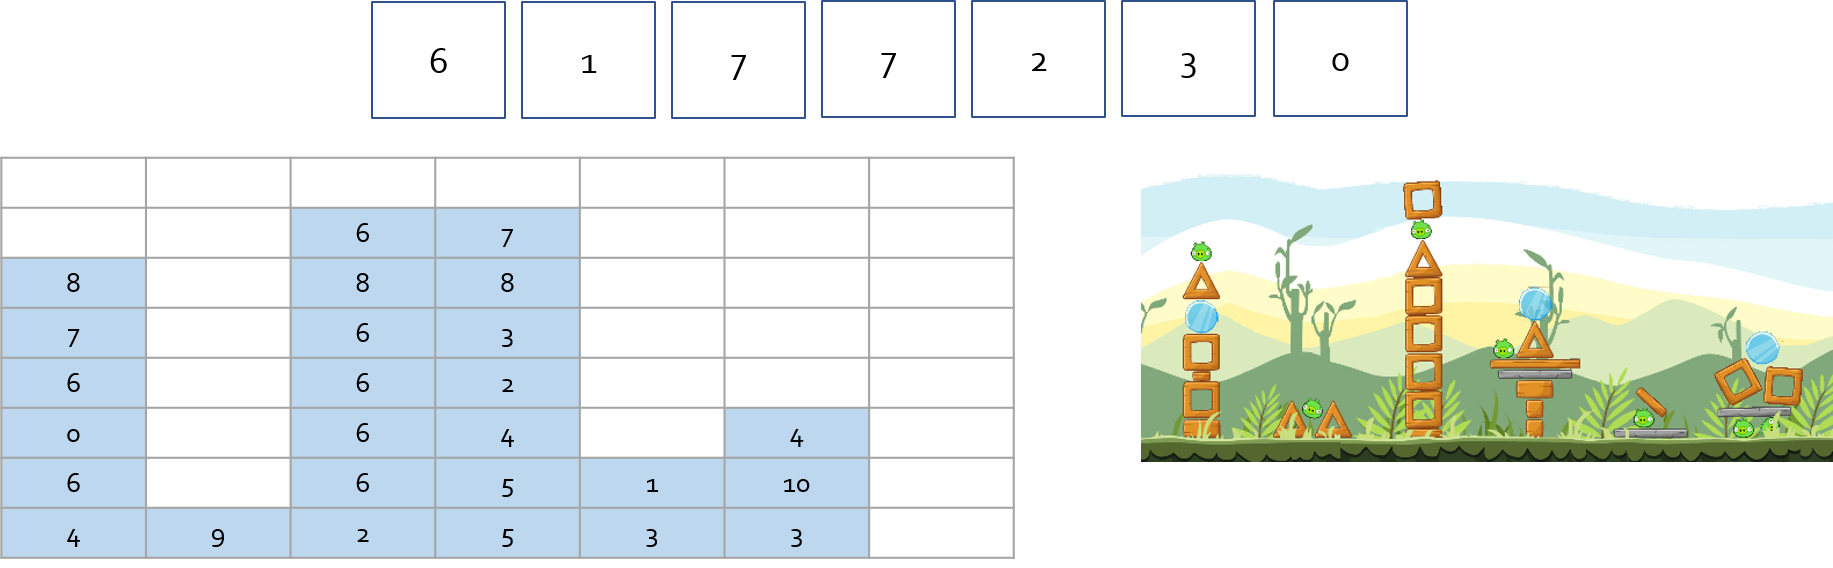
\includegraphics[width=80mm]{Images/mask_layer.png}}
        \caption{Mask array with column and fenotype representation.}
        \label{mask_layer}
    \end{figure}
    
    \begin{figure}[htbp]
        \centerline{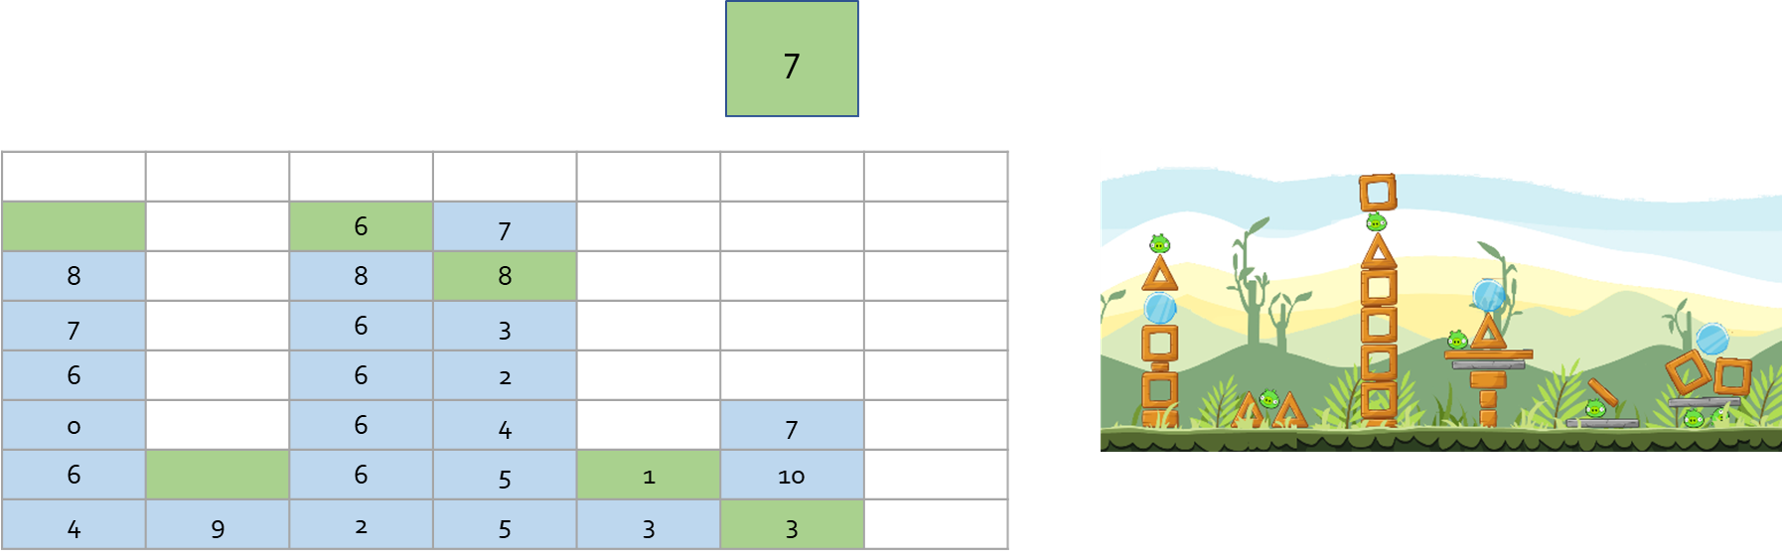
\includegraphics[width=80mm]{Images/enemy_layer.png}}
        \caption{Amount of pigs in a level, their location relative to the mask layer (green) and fenotype representation.}
        \label{enemy_layer}
    \end{figure}
    
    In order to select the parents of the next generation the parents are ordered by
    their fitness, then the system can choose between 2 options for the selection,
    tournament selection or roulette selection:
    
    \begin{itemize}
        \item Tournament selection: in order to select the parent by this method the
        system checks the amount of crossovers assigned, then calculates the ammount
        of parent required to compete in pairs, then by doing a descendent selection
        the slots for the tournament are filled and the winners are calculated in
        each group.
        \item Roulette selection: this method of selection was first decided to be
        used directly by giving a proportional amount of chances to be selected
        according to the fitness of a individual, however since one of the
        objectives is to obtain variety of levels the roulette must first be ranked
        in order to ensure that low fitness individuals can be selected as parents.
    \end{itemize}
    
    As for the crossover operations the system currently uses two types, single
    point crossover and double point crossover, however this crossover operation is
    not only applied to the piece array of an individual, but it is also applied to
    the mask of said individual, this way the mask can ensure that some pieces of
    some childs in the population are now placed in the level, this can bring the
    possibility that a mask that uses less pieces that it normally as can obtain a
    better fitness than one that uses all of them. An example of this two crossover
    types can be seen in figure \ref{crossover} in which the mask of an individual
    is combined with another and the resulting mask for the childs have different
    amount of pieces to be placed.
    
    \begin{figure}[htbp]
        \centerline{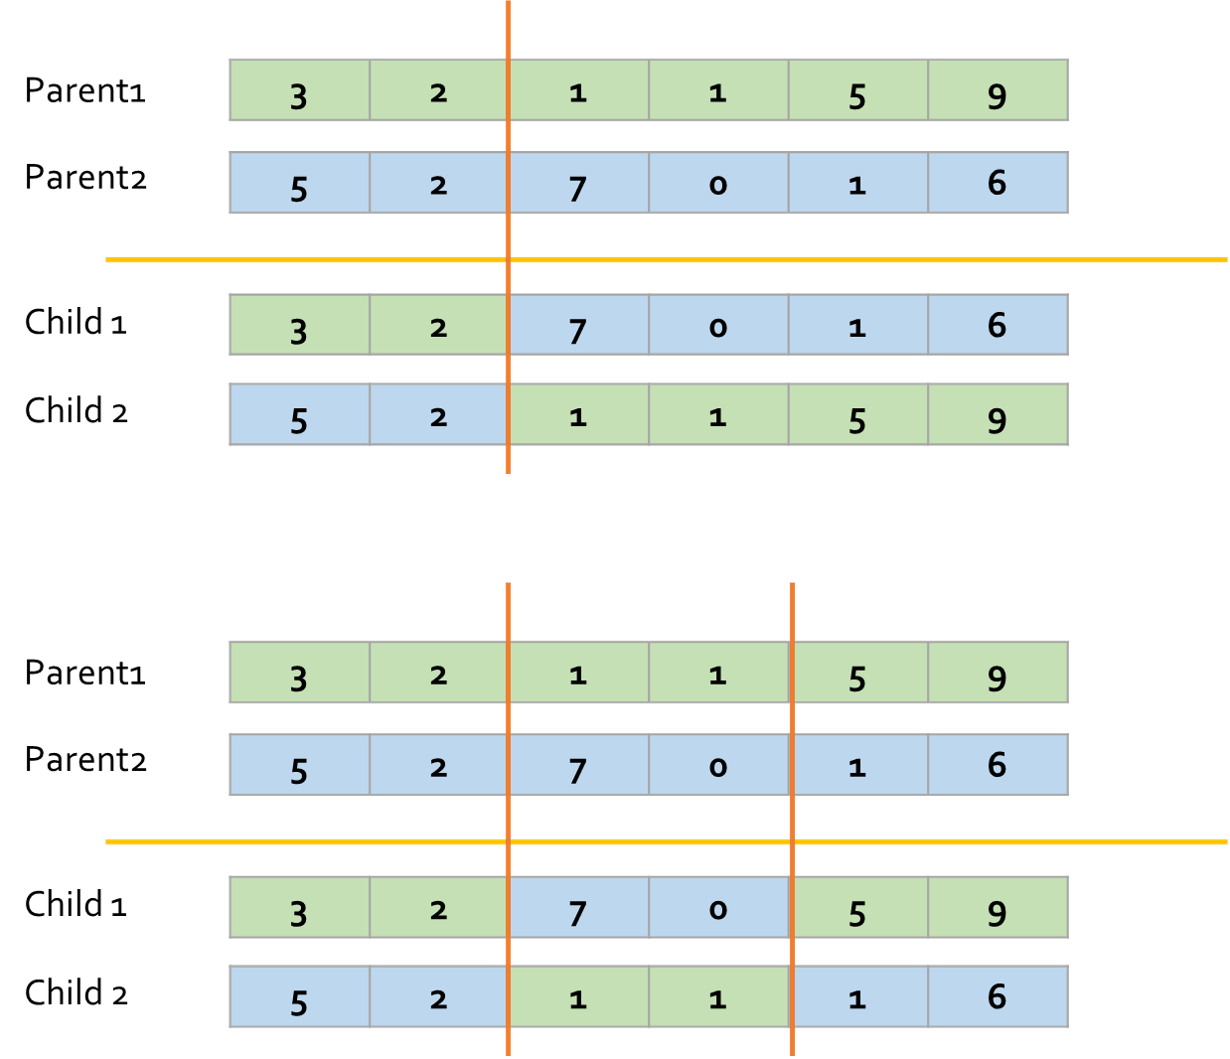
\includegraphics[width=80mm]{Images/crossover.png}}
        \caption{Single point crossover(up) and double point crossover(bottom) aplied to an individual mask.}
        \label{crossover}
    \end{figure}
    
    The mutation operations of the generator work with the pieces layer of an
    individual, the four types of mutations used are:
    
    \begin{itemize}
        \item Add or remove elements from the piece list
        \item Change the piece that is being used in a point of the list
        \item Change the material a piece is made offsets
        \item Change the x and y coordinates of a piece
    \end{itemize}
    
    This mutations do not have to be used all at once on a single individual but
    depending on the probabilities they can happen all at once, since most of the
    pieces on a individual are mostly the same type of material then at least the
    material mutation can occurr on all or most of the individuals to ensure that
    all levels will not have all the pieces with the same material which could
    render a level \textit{"boring"} by the fitness function.
    
    Since this group of mutations further ensures diversity in the populations a
    different way to evaluate the individuals is needed, by using the previous
    proposed method as a base a way to evaluate the \textit{"diversity"} and
    \textit{"uniqueness"} of a individual, for this we first remove the \textit{x}
    and \textit{y} position as well as the \textit{angle} errors in order to add two
    new evaluation formulas as follows:
    
    \begin{itemize}
        \item Hamming distance: a simle explanation for the \textit{Hamming
        distance} is that it is a calculation applied to a pair of strings where the
        objective is to find the minimum required number of substitutions required in
        order to convert a string exactly the same as the other, its formula is
        shown in equation \ref{hamming_distance}, since the formula itself locates
        the minimum number of substitutions then we compare the individual
        with the rest of the population trying to find the maximum number of
        substitutions required efectively using the formula to give a better fitness
        to those individuals that are different from the group.
        \item Shannon entropy: the shannon entropy is used on information theory to
        calculate the disorder or uncertainty, in this case it will be used to
        determine if a level is \textit{"boring"} or \textit{"interesting"} based on
        the amount of entropy calculated according to the pieces used in a level
        where a low entropy is boring because if a determined level as a lot of
        repeated pieces then it will look simple, the formula used is shown in
        equation \ref{shannon_entropy} where the elements calculated are the pieces
        of a level and their appearance probability against all others.
    \end{itemize}
    
    \begin{equation}
        \begin{aligned}
        d = min \left\{ \ d(x,y): x,y \in C, if \: x \neq y, 1 \: else \: 0 \: \right\} \
        \end{aligned}
        \label{hamming_distance}
    \end{equation}
    
    \begin{equation}
        \begin{aligned}
        S = - \Sigma_i P_i \log P_i
        \end{aligned}
        \label{shannon_entropy}
    \end{equation}
    
    Finally figure \ref{layer12_combine} and figure \ref{layer123_combine} represent 
    the way all the layers of an individual al combined to create a level after all 
    the selection, combination and mutation operations, first in figure \ref{layer12_combine}
    the composites layer is obtained from an individual, by a background process the 
    width and height of all composites are obtained, then using the mask from the same 
    individual the composites are placed in the order they are in their respective list 
    (left to right in the level) in case a mask is not able to accommodate all the 
    composites the remaining ones are not placed nor taken into account on the evaluation 
    process, in the opposite case that there are not enough composites to fill a mask 
    then the remaining areas are not taken into account as well, then in figure \ref{layer123_combine} 
    the previous combination of layers is evaluated by cheking which placed composites 
    can hold a pig in the center or on the top of it, then the pigs are placed in the 
    same oreder the composites are placed (left to right) in the locations where one 
    is able to be placed.
    
    \begin{figure}[htbp]
        \centerline{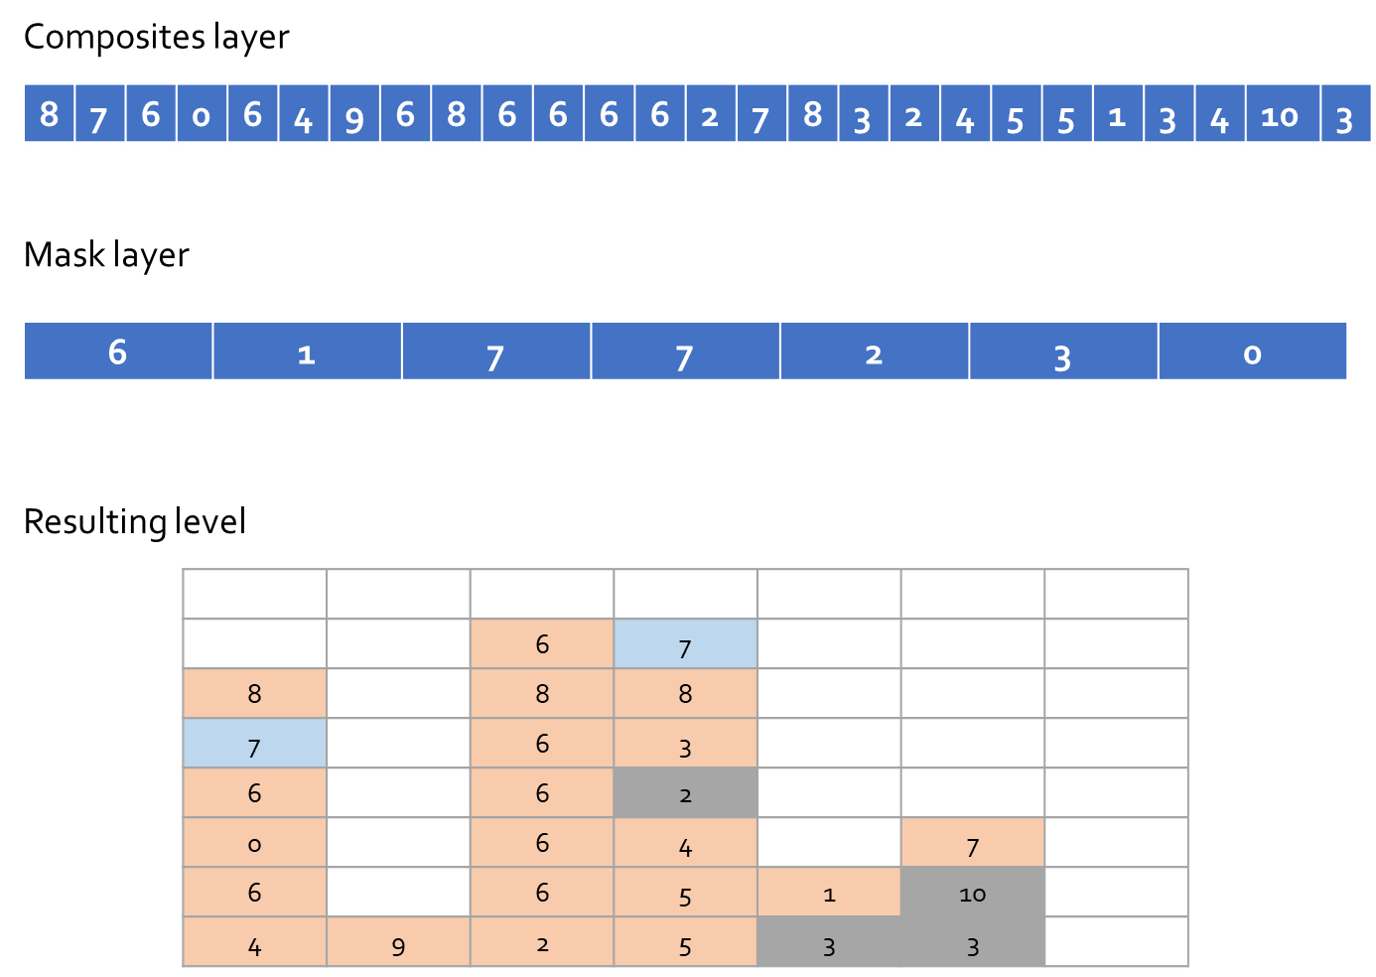
\includegraphics[width=80mm]{Images/layer12_combine.png}}
        \caption{Combination of composites layer and mask layer.}
        \label{layer12_combine}
    \end{figure}
    
    \begin{figure}[htbp]
        \centerline{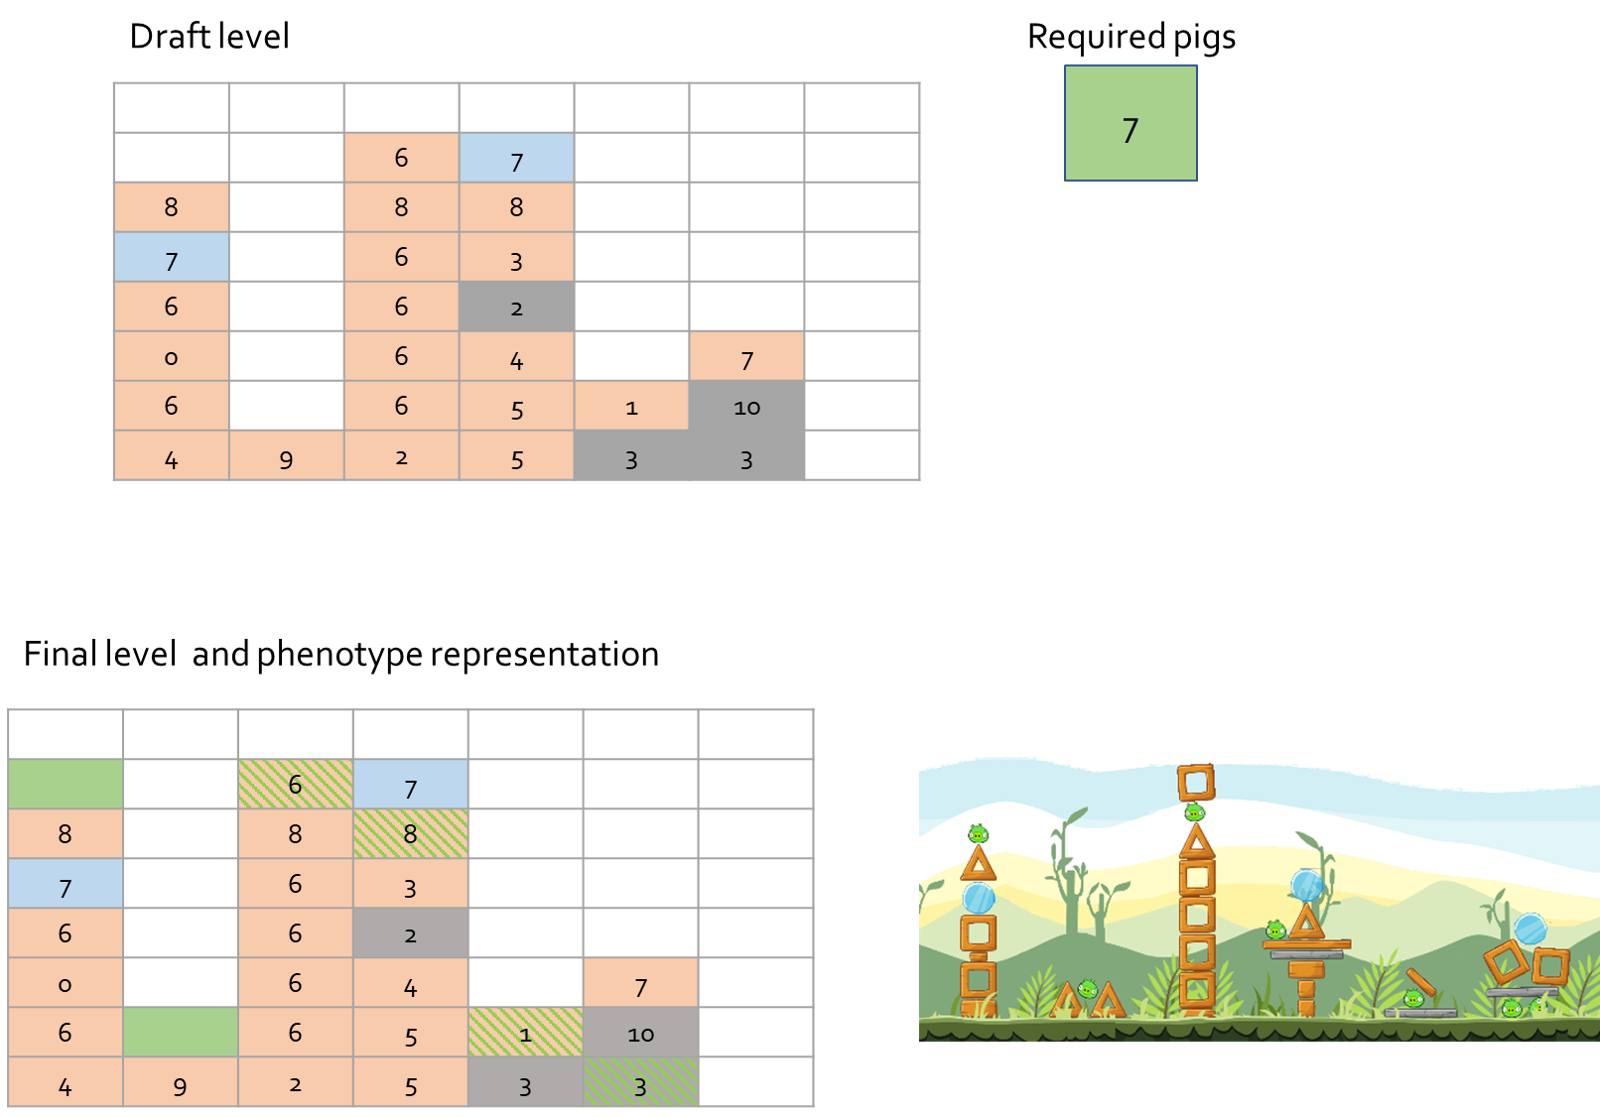
\includegraphics[width=80mm]{Images/layer123_combine.png}}
        \caption{Combination of figure \ref{layer12_combine} layers with pig layer.}
        \label{layer123_combine}
    \end{figure}
    
    Using all this configurations the system is capable of creating levels, some of
    them playable as shown in figure \ref{result_1} however the levels that can be
    generated are far from optimized to be played on, this is an issue that must be
    changed in future instances but the generator itself is able to be used as a
    base for a more complex one, and as shown in the future work section this issues
    can be solved by different means.
    
    \begin{figure}[htbp]
        \centerline{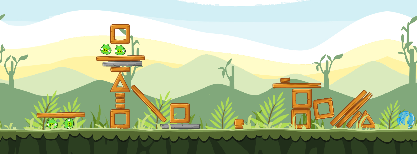
\includegraphics[width=80mm]{Images/Result_n2.png}}
        \caption{Example of resulting level with current system.}
        \label{result_1}
    \end{figure}
    
    \section{Conclusions and future work}
    
    The system as been able to generate levels that fulfill the requirements
     provided by the parameters file, however a way to evaluate that the levels
     generated are indeed \textit{"fun"} or \textit{"interesting"} is still needed,
     at this point we have two was to evaluate the results:
     \begin{itemize}
        \item User survey, in case a survey is used as an evaluation tool then first
        the system has to generate the levels and a group of people must participate
        by playing the levels and answering a set of questions afterwards, the
        questions themselves must try to capture the feeling of a person towards the
        game like questioning if a level was too easy or too dificult to solve, if
        the generated structures look interesting or if the level required them to
        strategize how to use the provided birds to solve the level, the survey must
        be applied to a equal quantity of people of three different game skill
        levels,\textit{"non video game players"}, \textit{"casual video game
        players"} and \textit{"avid video game players"}, this way we can evaluate a
        level or the entire system by knowing if all skill levels did not enjoyed a
        level because it was too simple or easy.
        \item By using a naive agent, if a naive agent is used to play the levels we
        can obtain data of how the agent solves the levels placed before them, and
        the way to evaluate if the level is or not \textit{"interesting"} will be by
        checking how easily the aggent is able to solve a level, the point here is
        to have a level that cannot be solved by a single movement but to have one
        that a human player has to think a while to solve tryingto place the
        difficulty of a level just at the middle point between easy and hard
        difficulty levels.
    \end{itemize}
    
    Other aspects that the system need to improve is in the processing time
    required, since the current way to calculate the fitness and create the next
    generations of a population the system requires the system to execute
    simulations of the levels on every generation that passes therefore increasing
    the time it takes to complete an entire cycle of execution, so in order to
    change this we require to create a way to evaluate a level using only the
    information of the pieces, locations and pigs locations and using this data to
    predict the way a level will behave when placed in a real simulation environment
    therefore drastically reducing execution times.
    
    Finally a different method to evaluate the individuals must be created, this is
    because the current evaluation method allows us to generate playable levels,
    this levels are far from ideal in the way that they only use a certain range of
    items present in the game therefore reducing the potential of a level, we expect
    to make the current fitness function work the most eficient that it can but
    another possible solution is found a good combination of formulas to generate
    the fitness function.

\bibliographystyle{IEEEtran}
\bibliography{References/article_references.bib}

\end{document}
